\begin{frame}
\frametitle{Why is this hard?}
\textbf{Qubits are large:} ``No other modes'' criterion difficult.
\begin{itemize}
    \item Modes in materials at $\omega_0$ cause decoherence.
    \item Electromagnetic modes on the chip (funny story)
    \item Crud on metal surface makes noisy magnetic field
\end{itemize}
\pause
\begin{columns}
  \begin{column}{0.4\textwidth}
    \begin{figure}
      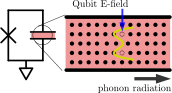
\includegraphics{tls.pdf}
    \end{figure}
  \end{column}
  \begin{column}{0.6\textwidth}
    \begin{itemize}
        \item Atomic defects couple to qubit: decoherence. 
        \item Defects in capacitor (old style) and junctions!
        \item Defects also on surface. Less coupled to qubit, but not zero.
    \end{itemize}
  \end{column}
\end{columns}
\pause
\textbf{Control wire density}
\begin{itemize}
    \item One wire per qubit. A million coaxial wires?!
    \item Thermal load on cryostat.
    \item Weight, cost, size
    \item How do we route the wires into the chip without dielectrics?
\end{itemize}
\end{frame}
